\section*{Experiment 2}
% Using the provided simulation code, generate a set of curves that show the tradeoffs between blocking probability, offered load (in Erlangs) and the number of channels. (Curves of this kind were presented earlier in class. See the “Circuit Switching Performance” lecture overheads.) Compare your results to that obtained using the Erlang B formula. According to Erlang B, the probability that a call is blocked is given by
% PB = AN /N ! ∑N i=0 Ai/i!
% where A is the offered load (in Erlangs) and is given by
% A = λh
% where λ is the call arrival rate (in calls per unit time, e.g., calls/minute), h is the average call holding time (in the same time units, e.g., minutes), and N is the total number of channels. Write a program to perform this computation (Feel free to use any programming language you want, e.g., Matlab, C, etc.) Include a listing of your program in your writeup. Check the results of your program using one of many online Erlang B calculators. Just google search for “Erlang B calculator”. Include the URL of the calculator that you used. The set of curves that show the tradeoffs between blocking probability, offered load (in Erlangs) and the number of channels can be seen in Figure~\ref{fig:exp2}. We can observe that the blocking probability decreases as the number of channels increase, and increasing the offered load will increase the blocking probability at a given number of channels.
The set of curves that show the tradeoffs between blocking probability, offered load (in Erlangs) and the number of channels can be seen in Figure~\ref{fig:exp2}. We can observe that the blocking probability decreases as the number of channels increase, and increasing the offered load will increase the blocking probability at a given number of channels.

When plotting these results with the Erlang B formula in MATLAB, we observe the same results with essentially identical curves as seen in Figure~\ref{fig:exp2_matlab}. The MATLAB code used to calculate the Erlang B formula can be seen in Listing~\ref{list:exp2}. We compared several of our results of from our program with an \href{https://owenduffy.net/traffic/erlangb.htm}{online Erlang B calculator} and had matching results. For example, for $A = 5, N = 10$, both calculated $P_B = 0.184$. 

\begin{lstlisting}[style=Matlab-editor,firstnumber=3,caption=Erlang B Formula, label=list:exp2]
syms k

for A = 1:20
	for N = 1:20
		PB(A,N) = ((A^N)/factorial(N))/symsum(A^k/factorial(k),k,0,N);
	end
end
\end{lstlisting}

\begin{figure}[htp]
\centering
\captionsetup{justification=centering}
\begin{tikzpicture}
	\begin{axis}
		[
		title = {Blocking Probability vs. Number of Channels for Various Offered Loads},
		width = 0.969\textwidth,
		%height = 150,
		xmin = 1, xmax = 20, xtick={1,...,20},
		ymin = 0.0001, ymax = 1, ymode=log, log basis y = {10},
		ylabel = Blocking Probability, xlabel = Number of Channels,
		xticklabel style={
			/pgf/number format/fixed,
			/pgf/number format/precision=3
		},
		scaled x ticks=false,
		% legend pos=outer north east,
		legend style={at={(0.5,-0.1)},anchor=north},
		legend columns=5,
		% legend style={font=\scriptsize}
		% some code for adding points
		%nodes near coords={%
		%\footnotesize
		%$(\pgfmathprintnumber
		%{\pgfkeysvalueof{/data point/x}},
		%\pgfmathprintnumber
		%{\pgfkeysvalueof{/data point/y}})$%
		%},
		]
		\addlegendimage{empty legend}
		\addlegendentry{\makebox[0pt][l]{\hspace{1.6cm}Offered Load (Erlangs)}}
		\addlegendimage{empty legend}
		\addlegendentry{}
		\addlegendimage{empty legend}
		\addlegendentry{}
		\addlegendimage{empty legend}
		\addlegendentry{}
		\addlegendimage{empty legend}
		\addlegendentry{}
		\addplot+ [mark=o, thick] table [y=$block1$, x=$num_chan$]{./data/exp2.dat};
		\addlegendentry{$a = 1$}
		\addplot+ [mark=o, thick] table [y=$block2$, x=$num_chan$]{./data/exp2.dat};
		\addlegendentry{$a = 2$}
		\addplot+ [mark=o, thick] table [y=$block3$, x=$num_chan$]{./data/exp2.dat};
		\addlegendentry{$a = 3$}
		\addplot+ [mark=o, thick] table [y=$block4$, x=$num_chan$]{./data/exp2.dat};
		\addlegendentry{$a = 4$}
		\addplot+ [mark=o, thick, cyan, solid] table [y=$block5$, x=$num_chan$]{./data/exp2.dat};
		\addlegendentry{$a = 5$}
		\addplot+ [mark=o, thick, yellow, solid] table [y=$block6$, x=$num_chan$]{./data/exp2.dat};
		\addlegendentry{$a = 6$}
		\addplot+ [mark=o, thick, pink, solid] table [y=$block7$, x=$num_chan$]{./data/exp2.dat};
		\addlegendentry{$a = 7$}
		\addplot+ [mark=o, thick, orange, solid] table [y=$block8$, x=$num_chan$]{./data/exp2.dat};
		\addlegendentry{$a = 8$}
		\addplot+ [mark=o, thick, teal, solid] table [y=$block9$, x=$num_chan$]{./data/exp2.dat};
		\addlegendentry{$a = 9$}
		\addplot+ [mark=o, thick, purple, solid] table [y=$block10$, x=$num_chan$]{./data/exp2.dat};
		\addlegendentry{$a = 10$}
		\addplot+ [mark=o, thick, lime, solid] table [y=$block11$, x=$num_chan$]{./data/exp2.dat};
		\addlegendentry{$a = 11$}
		\addplot+ [mark=o, thick, olive, solid] table [y=$block12$, x=$num_chan$]{./data/exp2.dat};
		\addlegendentry{$a = 12$}
		\addplot+ [mark=o, thick, magenta, solid] table [y=$block13$, x=$num_chan$]{./data/exp2.dat};
		\addlegendentry{$a = 13$}
		\addplot+ [mark=o, thick, gray, solid] table [y=$block14$, x=$num_chan$]{./data/exp2.dat};
		\addlegendentry{$a = 14$}
		\addplot+ [mark=o, thick, Emerald, solid] table [y=$block15$, x=$num_chan$]{./data/exp2.dat};
		\addlegendentry{$a = 15$}
		\addplot+ [mark=o, thick, YellowGreen, solid] table [y=$block16$, x=$num_chan$]{./data/exp2.dat};
		\addlegendentry{$a = 16$}
		\addplot+ [mark=o, thick, Periwinkle, solid] table [y=$block17$, x=$num_chan$]{./data/exp2.dat};
		\addlegendentry{$a = 17$}
		\addplot+ [mark=o, thick, Melon, solid] table [y=$block18$, x=$num_chan$]{./data/exp2.dat};
		\addlegendentry{$a = 18$}
		\addplot+ [mark=o, thick, PineGreen, solid] table [y=$block19$, x=$num_chan$]{./data/exp2.dat};
		\addlegendentry{$a = 19$}
		\addplot+ [mark=o, thick, RoyalPurple, solid] table [y=$block20$, x=$num_chan$]{./data/exp2.dat};
		\addlegendentry{$a = 20$}
	\end{axis}
\end{tikzpicture}
\caption{Experiment 2: Simulation}
\label{fig:exp2}
\end{figure}

\begin{figure}
\centering
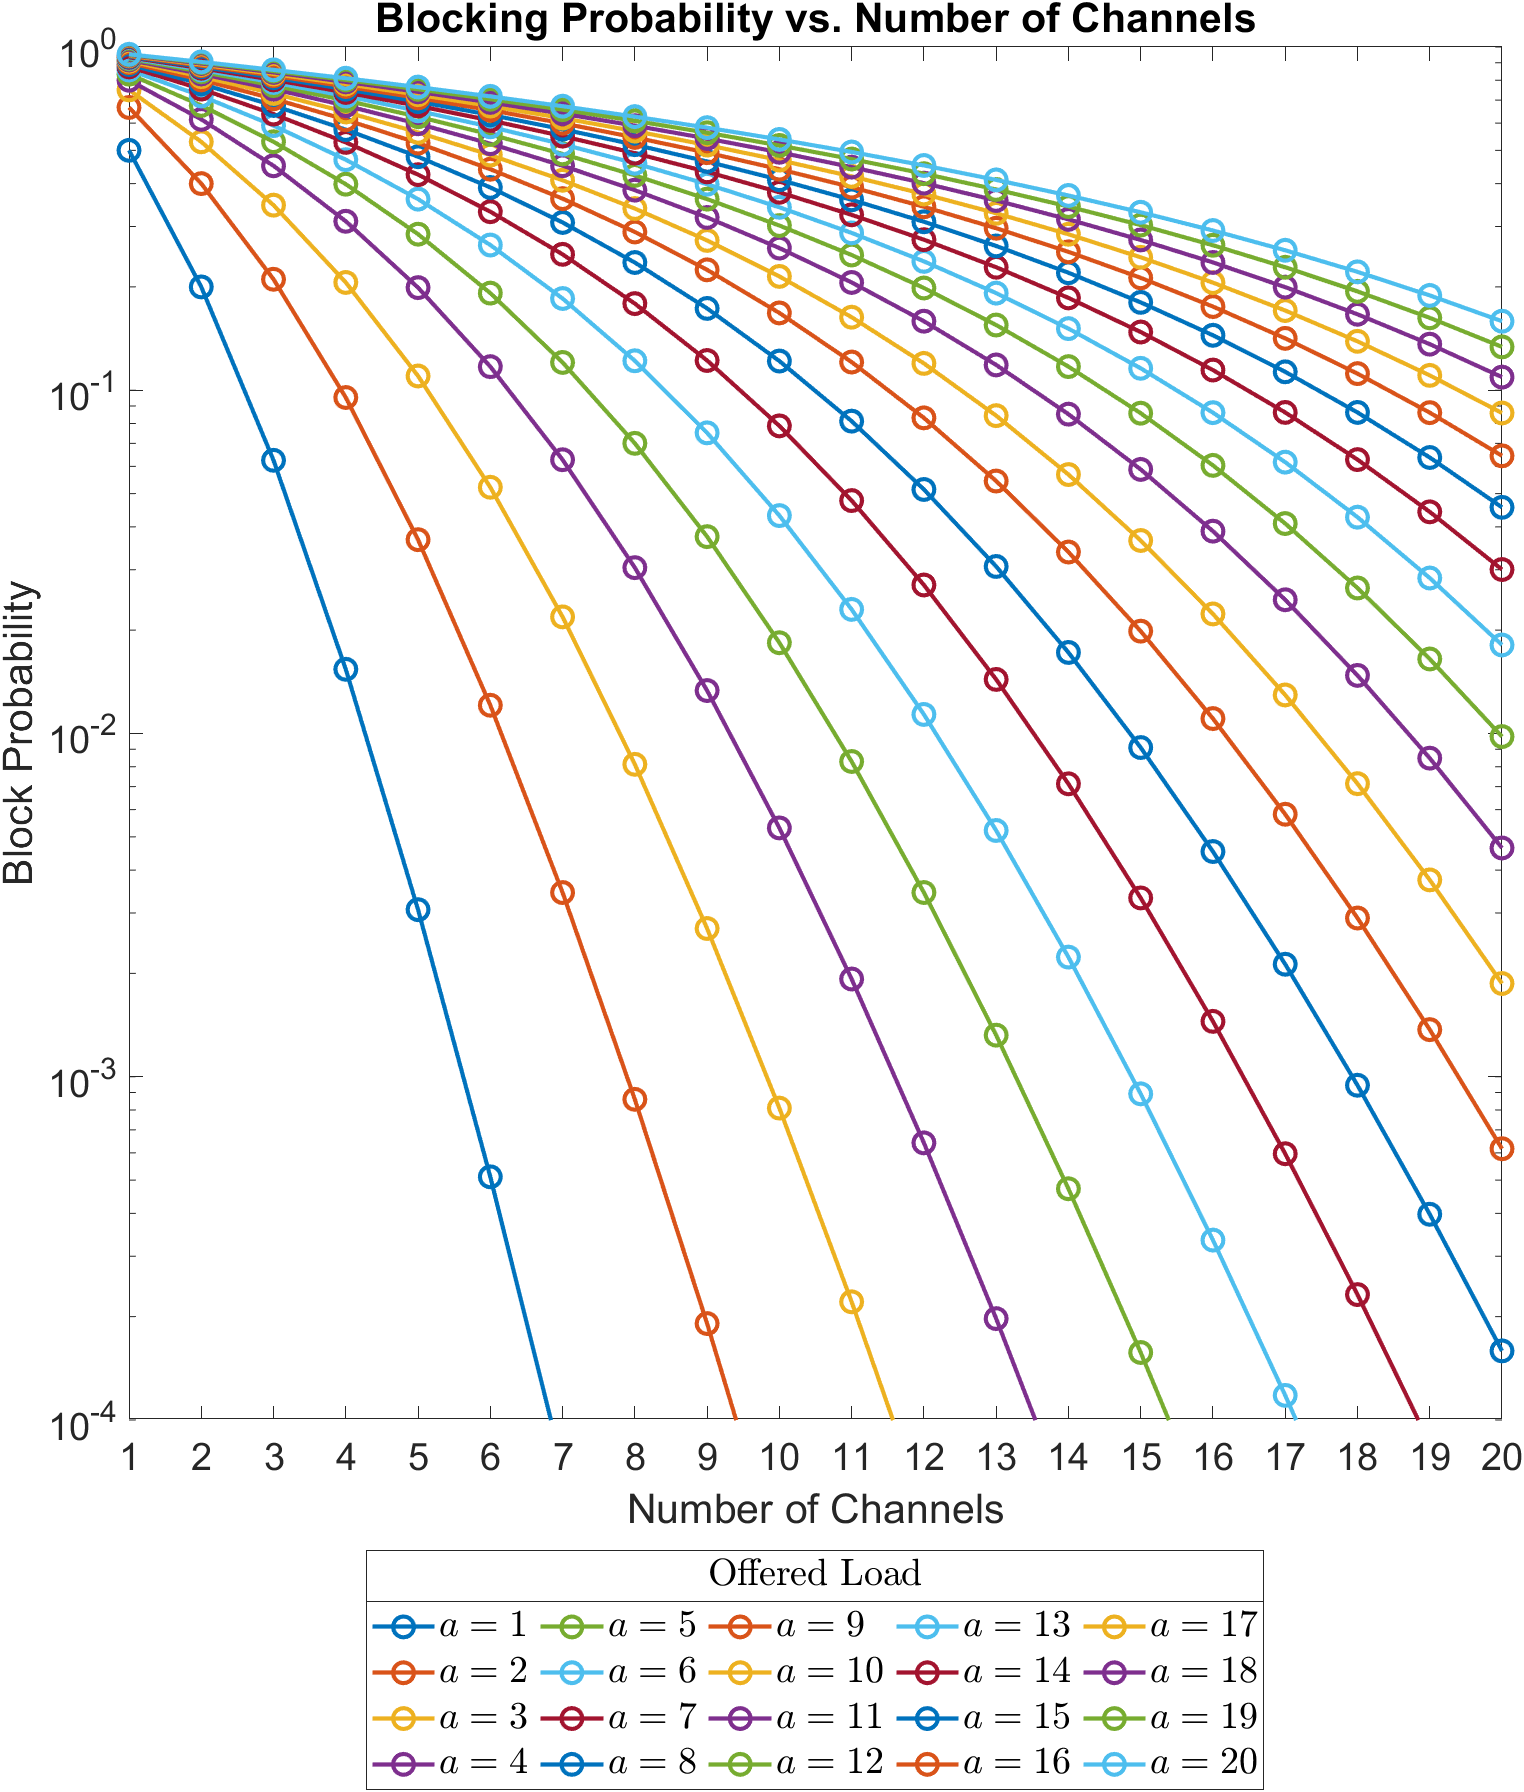
\includegraphics[width=\textwidth]{exp2.png}
\caption{Experiment 2: MATLAB}
\label{fig:exp2_matlab}
\end{figure}